\section{Conclusions}

\begin{frame}{Conclusions}
\only<1-2>
{
  \begin{block}{Résultats}
  \begin{itemize}
  \item Test automatique,
  \item Retour granulaire,
  \item Aspect ludique qui émerge du retour d'informations.
  \end{itemize}
  \end{block}
}
\only<2>
{
  \begin{alertblock}{Problèmes}
  \begin{itemize}
  \item Trop de temps passé dans les menus,
  \item Le patient regarde le membre,
  \item Le retour incite à forcer.
  \end{itemize}
  \end{alertblock}
}
\only<3-4>
{
  \begin{alertblock}{Limites}
  \begin{itemize}
  \item Précision insuffisante,
  \item Rotations déduites des positions,
  \item Zigfu.
  \end{itemize}
  \end{alertblock}
}
\only<4>
{
  \begin{block}{Ouverture}
  \begin{itemize}
  \item Poursuite de l'étude en stage~:
  \begin{itemize}
  \item \textbf{Geoffrey~:} paramétrage thérapeutique de jeu,
  \item \textbf{William~:} meilleure extraction de squelette. 
  \end{itemize}
  \end{itemize}
  \end{block}
}
\end{frame}

\section{Stage}

\begin{frame}{Projet principal}
\begin{block}{``Hammer And Planks''}
\begin{itemize}
\item interface thérapeutique,
\item multiple péripheriques de contrôles.
\end{itemize}
\end{block}
  \begin{center}
    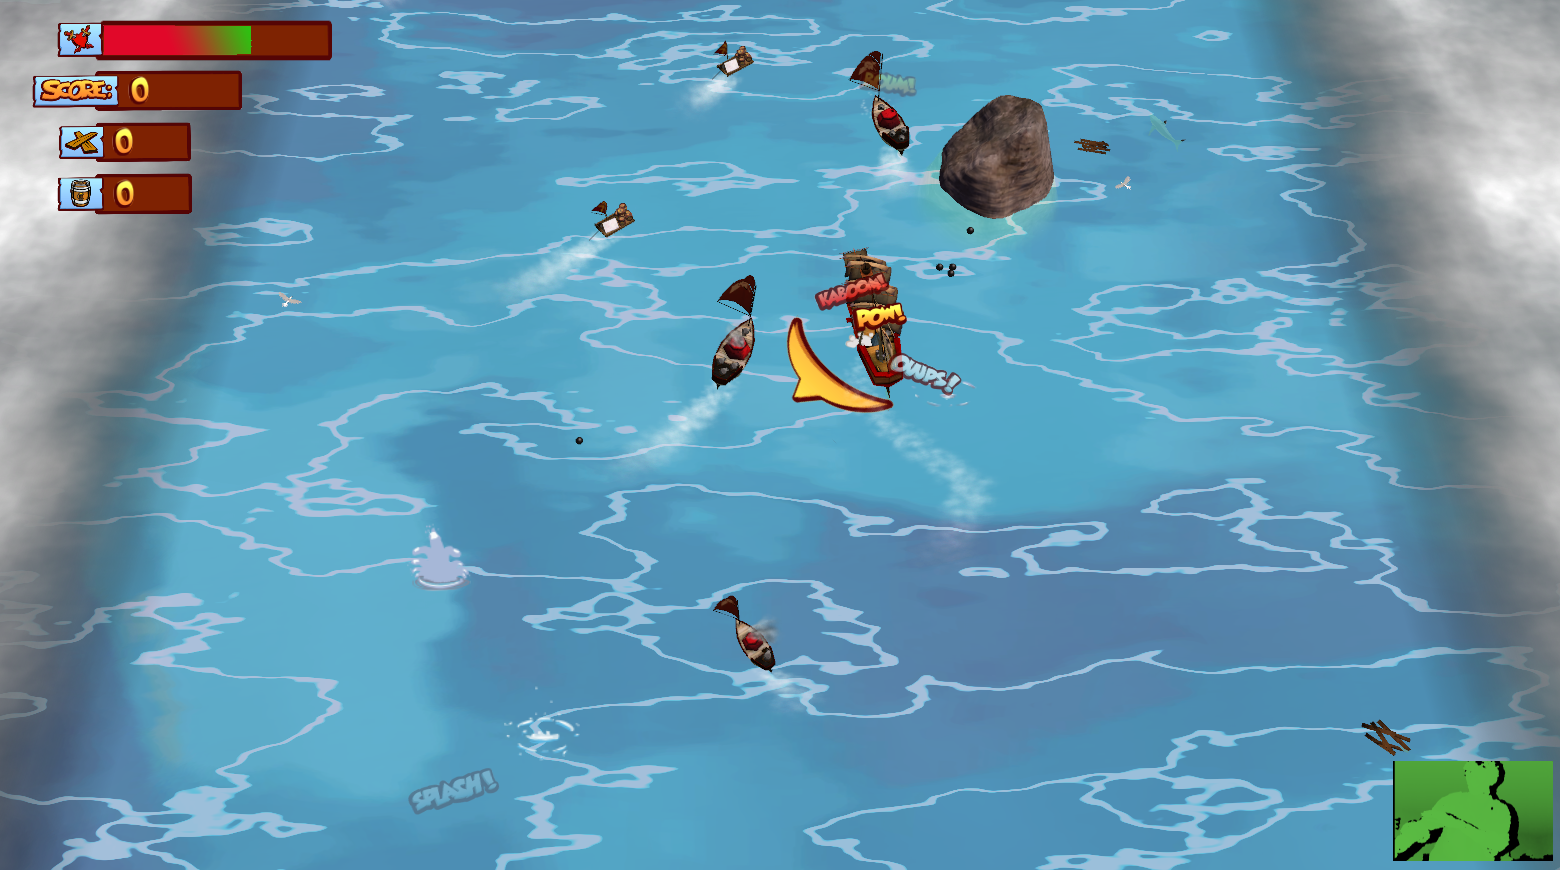
\includegraphics[height=0.5\textheight]{../images/hnp}
  \end{center}
  \vfill

\end{frame}

\begin{frame}{``Game Jam''}
\begin{block}{``Stickman Judgement Day''}
\begin{itemize}
\item jeu Kinect fait en une semaine,
\item adaptation thérapeutique envisageable\ldots
\end{itemize}
\end{block}

  \begin{center}
    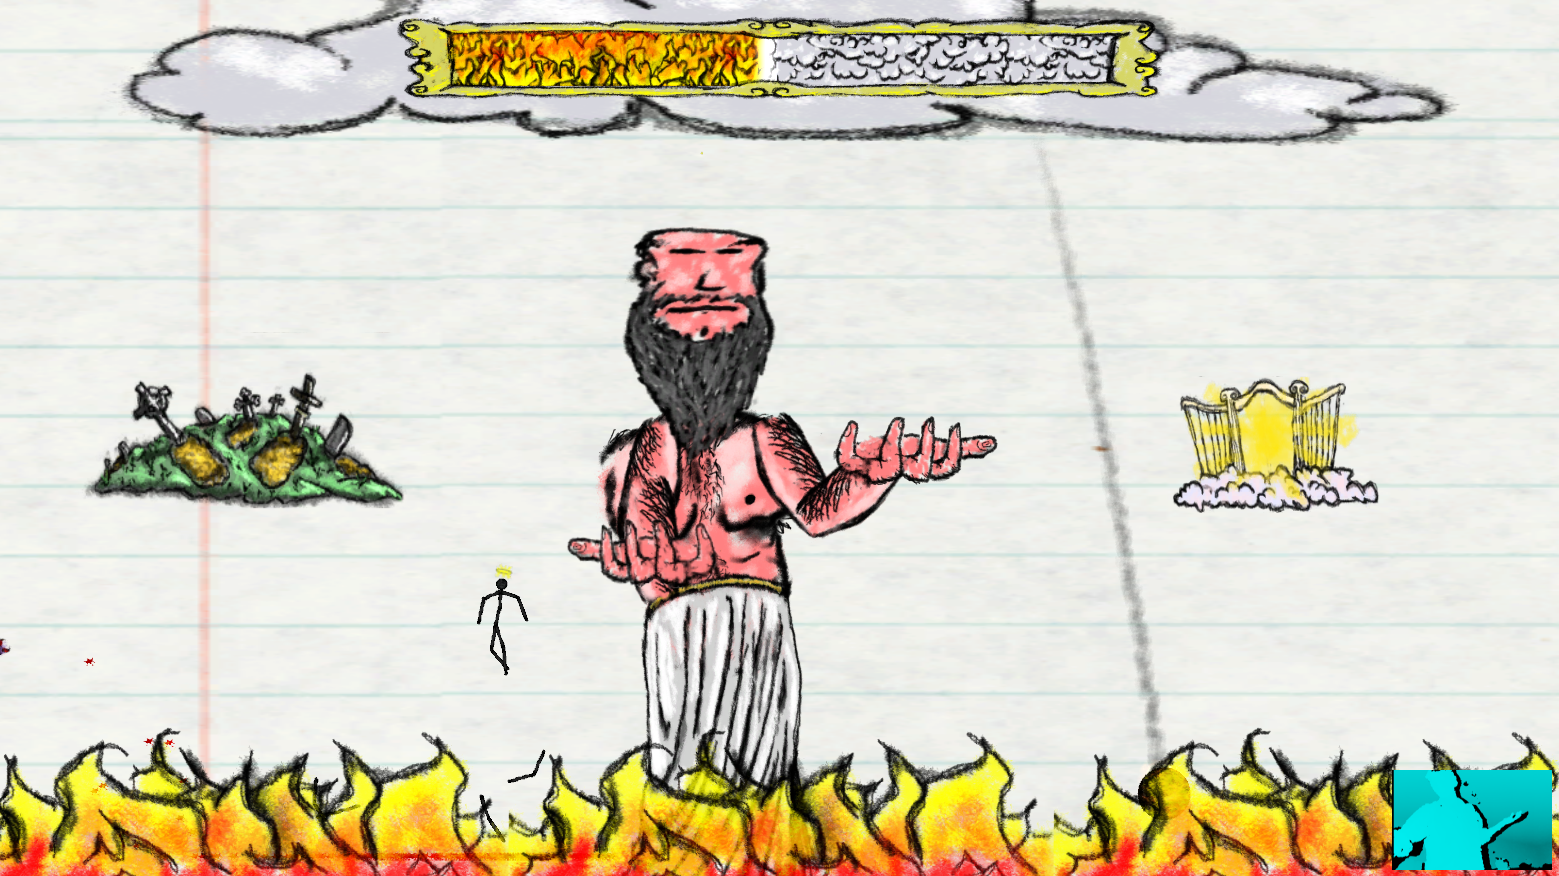
\includegraphics[height=0.5\textheight]{../images/leminect}
  \end{center}
  \vfill

\end{frame}